%% V1.0
%% by Shingo Mori, spawn.s.mori@gmail.com

\documentclass[10pt,journal,compsoc]{IEEEtran}

\usepackage[pdftex]{graphicx} 
\usepackage{cite}
\usepackage{subfig}
\hyphenation{op-tical net-works semi-conduc-tor}

\begin{document}

\title{Robotic Inference Writeup}

\author{Shingo Mori}

\markboth{Inference project, Robotic Nanodegree, Udacity}%
{}
\IEEEtitleabstractindextext{%

\begin{abstract}
In this project, prototypes of neural network is built on the supplied data and my own collected data to classify objects in a scene. Networks are trained and tested using the NVIDIA DIGITS workspace. A CNN is trained on the supplied data set to classify objects placed on a conveyor belt. Another CNN is trained on the collected data to classify garbage. The accuracy and the inference time of the network for the supplied data meet the requirement.
\end{abstract}

\begin{IEEEkeywords}
Object Classification, Udacity, NVIDIA DIGITS, CNN.
\end{IEEEkeywords}}


\maketitle
\IEEEdisplaynontitleabstractindextext
\IEEEpeerreviewmaketitle
\section{Introduction}
\label{sec:introduction}

\IEEEPARstart{A} common problem in Robotics is  the recognition of objects from a live camera video feed. Both speed and accuracy is required for a robot to perform object recognition in a real environment. Suppose building an intelligent waste bin which automatically separates recyclable garbage and other garbage. Poor accuracy and inference time may frustrate users. Thus, an accurate and fast network working on a limited resource of IoT device is necessary for good user experience. Using deep neural net on GPU makes this possible by allowing a robot to build an efficient recognition pipeline.

Since developing a deep neural network for optimal results require a lot of effort and time, being able to rapidly prototype a network is necessary. The NVIDIA DIGITS work flow makes this possible by providing us an interface that simplifies the task of training the network and testing the performance of its inference process.

In this project, we assume that NVIDIA Jetson TX1/TX2 will be used an embedded system.

\section{Background / Formulation}
The NVIDIA DIGITS workspace provide three types of deep neural network (LeNet, AlexNet, and GoogleNet) as standard models for image classification. After a few experiments done on the workspace, the result showed the inference time of all the three networks were faster than the requirement, and the accuracy of GoogleNet was the best. Another experiment shows that the performance of GoogleNet in terms of efficiency (accuracy per operation) is one of the best. \cite{DBLP:journals/corr/CanzianiPC16} Thus, GoogleNet is chosen as the network for the supplied data.

Parameters are determined experimentally. SGD for optimizer, 0.001 for base learning rate, 30 for epoch, were chosen.

Network and parameters used for the collected dataset are the same as those used for the supplied dataset.

\section{Data Acquisition}

\begin{figure}[thpb]
      \centering
      \subfloat[supplied dataset (from Udacity)]{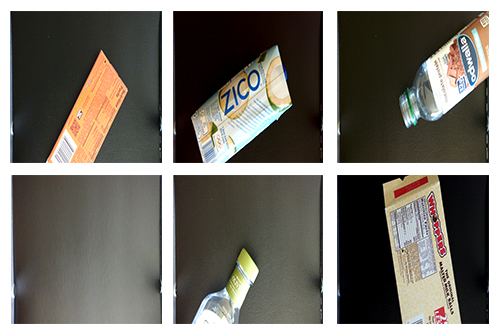
\includegraphics[width=0.9\linewidth]{data-p1-digits}\label{fig:supplied_data}}
      \vfill
      \subfloat[collected dataset]{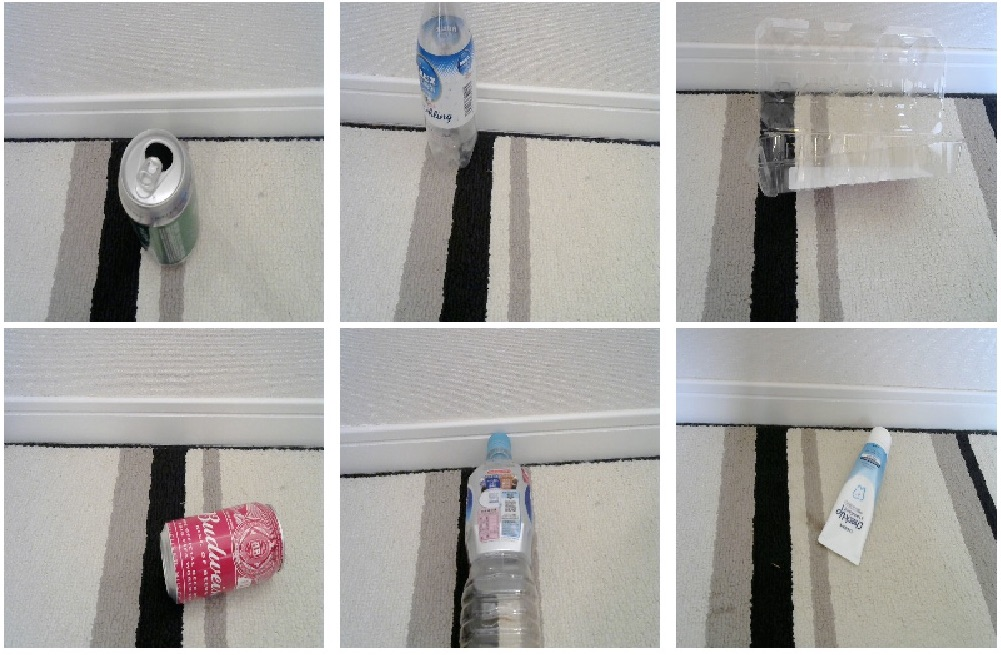
\includegraphics[width=0.9\linewidth]{data-p1-own}\label{fig:collected_data}}
      \caption{Example images of the dataset.}
\end{figure}

\subsection{Supplied Dataset}
The supplied dataset consists of photos taken from a Jetson mounted over a conveyor belt. There are three categories of photos: bottle (4568 images), candy box (2495 images), and nothing (3031 images). Each photo is a 8-bit RGB PNG image with the size of 500x500. Example images of photos taken by Udacity \cite{udacity:supplied_data} are shown in Fig. \ref{fig:supplied_data}.

The dataset is provided inside the NVIDIA DIGITS workspace by Udacity. The supplied dataset is used only as a training set. Test set is not directly provided to students.

\subsection{Collected Dataset}
The dataset is collected with a USB camera placed on a floor carpet. Photos of objects taken with different poses and positions are categorized into three types: can (7 objects, 227 images), plastic bottle (6 objects, 203 images), and other (18 objects, 217 images). 
Each photo is a 8-bit RGB PNG image with the size of 256x256.  Example images  are shown in Fig. \ref{fig:collected_data}.

75\% of the collected dataset is used as a training set and 25\% of it is used as a test set. The training set is augmented by creating vertically/horizontally flipped images of the original photos.

\section{Results}
\subsection{Supplied Dataset}
The accuracy of the network on the training set scored almost 100\%, as shown in Fig. \ref{fig:lac-sup}.

An 'evaluation' command provided by Udacity was used for testing the network. The maximum inference time was 8.4ms and the accuracy was 75.4\%, which meet the numerical requirements of 10ms and 75\%, respectively.

\subsection{Collected Dataset}
The accuracy of the network on the training set was around 92\% as Fig. \ref{fig:lac-own} shows.

The network was tested on the NVIDIA DIGITS. Number of images in the test set  correctly classified by the network were 212 out of 226 for can, 169 out of 202 for plastic bottle, and 216 out of 216 for other. The overall accuracy scored 92\%.

Inference time is not measured on the collected dataset. 

\begin{figure}[thpb]
      \centering
      \subfloat[supplied dataset]{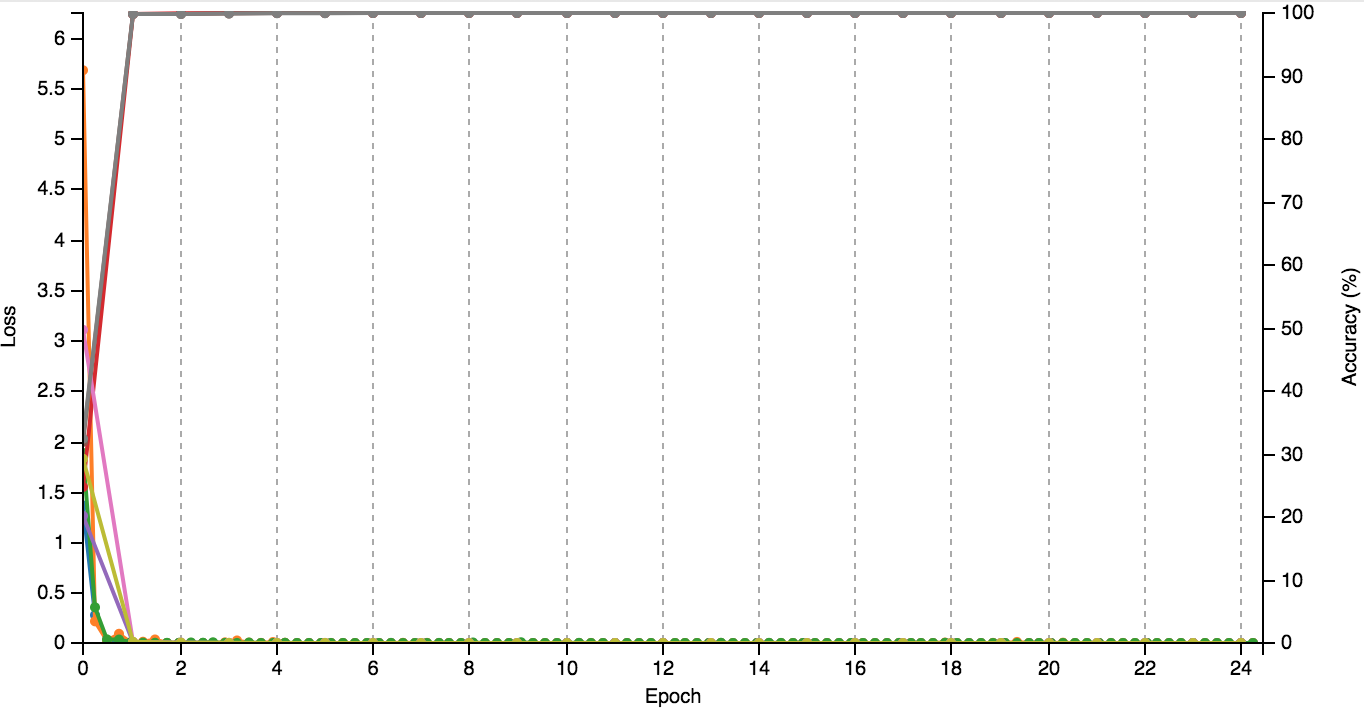
\includegraphics[width=0.9\linewidth]{loss-accuracy-curve-supplied}\label{fig:lac-sup}}
      \vfill
      \subfloat[collected dataset]{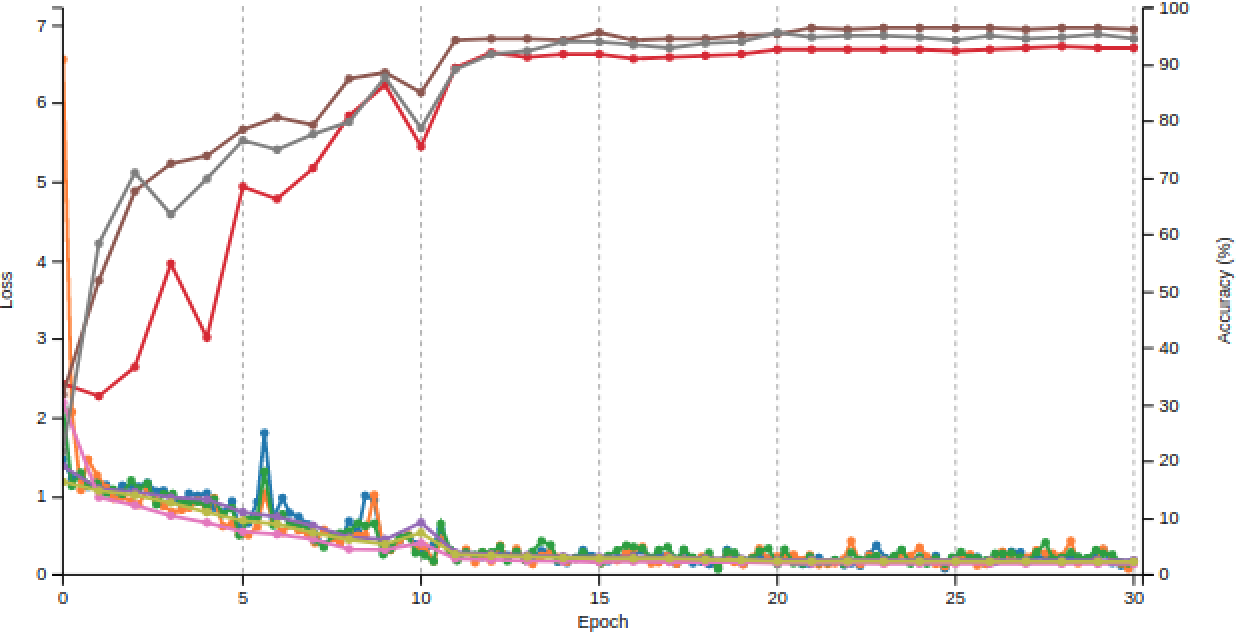
\includegraphics[width=0.9\linewidth]{loss-accuracy-curve-own}\label{fig:lac-own}}
      \vspace{0.5cm}
      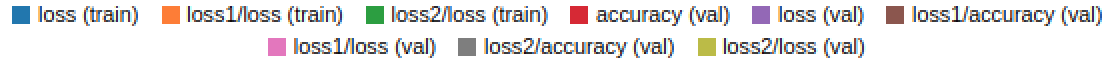
\includegraphics[width=\linewidth]{loss-accuracy-curve-legend}
      \caption{Loss and accuracy curves.}
\end{figure}

\section{Discussion}
\subsection{Supplied Dataset}
There is almost no difference between the training accuracy and the validation accuracy. However, a larger difference of around 17\% between the training accuracy and the test accuracy is observed. This increased difference indicates that although the network is not overfitting withing the training and validation set, it fails to generalize and performs poorly on the test set. This may be because there is a gap between the training/validation set and test set in terms of the variation of images. Some basic and advanced data augmentation techniques \cite{DBLP:report/Jason16} may solve this situation.

\subsection{Collected Dataset}
The network performs well both on the training set and the test set. Being able to classify garbage with the accuracy of more than 90\% may satisfy users.  However, this result does not guarantee that the network performs the same in real use. Although all the photos are taken from different poses and positions, the same objects are used for the training and test set, which means that the test set contains only the objects that are 'already seen' by the network. The accuracy may drop if the network performs classification on images of 'unseen' objects.

\section{Conclusion / Future work}
Prototypes of neural network is built on the supplied data and the collected data to classify objects in the scene. The accuracy and the inference time of the network for the supplied data meet the requirement. The accuracy of the network for the collected data is satisfactory within this project. However, its performance may drop on images of 'unseen' objects.

Future work may include testing on images with more variable objects, and measuring the inference time on actual device such as NVIDIA Jetson TX2.

\bibliography{bib}
\bibliographystyle{ieeetr}

\end{document}